\documentclass{article}

\usepackage{graphicx}
\RequirePackage{mathspec}
\RequirePackage{fontspec}
\RequirePackage{xunicode}
\RequirePackage[no-sscript]{xltxtra}
\RequirePackage{polyglossia}
\setdefaultlanguage{english}

\RequirePackage{microtype}

\title{Introduction to LaFiC}
\author{Sebastian Meisel}

\begin{document}

\maketitle


LaFiC means \textit{layout and format in comments}, as all layout and
format information is put into comment lines. So layout and
content are \emph{fully} separated.

\part{Installation}

Get source from github using:

\begin{verbatim}
git clone https://github.com/SebastianMeisel/lafic.git

\end{verbatim}

Add lafic directory to \$PATH, e.g.:

\begin{verbatim}
export PATH=${PATH}:~/lafic

\end{verbatim}

See \texttt{lafic-mode.el} for installation instructions, if you want
to use in in Gnu Emacs.

\part{Writing text in LaFiC}

\section{Lines and paragraphs}

The content is presented in two forms, which also include
the most basic layout: There are \emph{lines} and \emph{paragraphs}.

The difference is not so much the length, but lines include
none of the punctation marks ».«, »?«, »!«, \emph{»:«}. If no
further layout information is provided, these are
interpreted as headings.

The \emph{first} line is interpreted as \emph{the} title and presented as
this is as <h1>, when converted to Html, and \textbackslash title, when 
converted to \LaTeX.

Further line will be converted to <h3> (Html) or \textbackslash section
(\LaTeX), if no otherwise specified.

This way simple Documents Html may be structured with no explicit
layout information at all.

\section{Comments}

You can add comments to your text, by starting a single line
or each \emph{line} of a paragraph with a \% char with no leading
spaces. These lines or paragraphs must, however, be
separated by empty line from the content.

\begin{verbatim}
  % This is a comment.

  % This is a longer comment, that spreads over several
  % lines. It is important that it is not connected to a line
  % of the general content.

\end{verbatim}

“It is recommended, however, to start comments with two \% chars.
Else there may occur ‘ problems’, when there” is a »:« somewhere
in the comment. You also can start a longer comment this way
and don't need to repeat it ‘ in every’ line.

\begin{verbatim}
  %% This is a comment! No mistake!
  Even when you go on with no leading % it's still a comment.

\end{verbatim}


\section{Formated paragraphs}

Paragraphs can be formated by adding a line before the
paragraph, that starts with a \% char, followed by a single
word. There are some predefined keywords, like quote or
quotation for – well a quotation.

\begin{verbatim}
  % quote
  This is a quotation.

\end{verbatim}

\begin{quote}
This is a quotation.

\end{quote}

If the keyword is unknown, it will be converted to an environment
name in \LaTeX or the name of a <div> in Html.

\section{Formated lines}

Line are formated in the same way, only they are converted
to macros (\LaTeX) oder <span> names (HTML). Know keywords
are H1~… H6~for headings.

\begin{verbatim}
  % heading4
  This is a subsection

\end{verbatim}

\subsection{This is a subsection}

\section{Inline formation}

If you want to format words or sequences in a paragraph (or
line if needed), you add format lines with a leading \% after
a paragraph. It has two parts:

\begin{enumerate}

\item the word or the sequence to be formated in the form
  start…end. 
\item a keyword.

\end{enumerate}

The both are separated by a »:«.

Known environment keywords are e.g. quote or quotation.

If the keyword is unknown, it is converted to a macro
(\LaTeX) oder <span> (HTML) name.

\section{Images}

The simplest way to put an image into a LaFiC file is a
line with the image name, with a know extention: png, jpg,
jpeg, gif.

\begin{verbatim}
  Image.png
  % height = 40%

\end{verbatim}

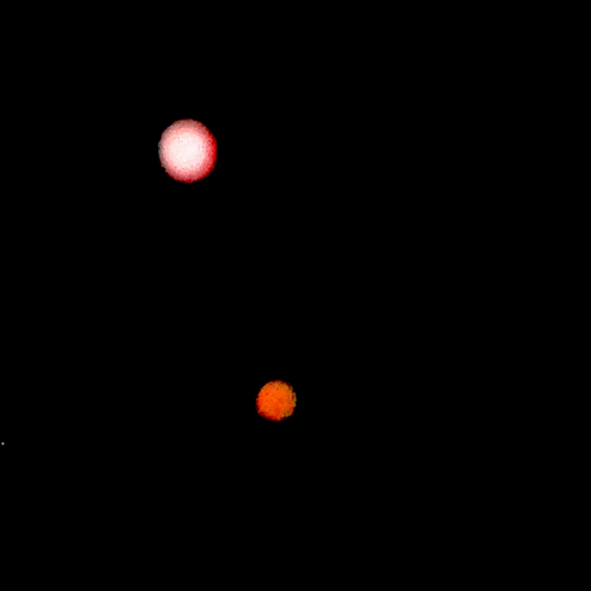
\includegraphics[height=.40\textheight]{Image.png}

Note that this will not put an figure environment in \LaTeX
files, so the image won't float this way. For this to
achieve to have to put \% image, \%img or \%figure before the
line. You don't need the extention then.

\begin{verbatim}
  %image
  Image.png
  % width = 40%
  % caption = "Moon and Mars"

\end{verbatim}

\begin{figure}[hbt]
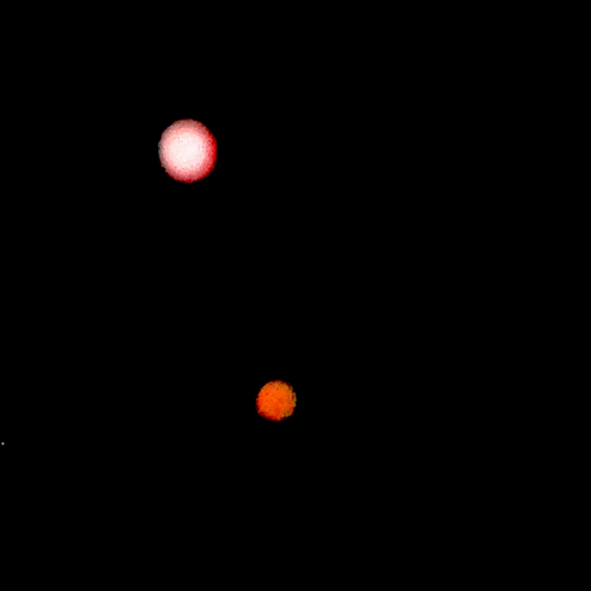
\includegraphics[width=.40\linewidth]{Image.png}
\caption{"Moon and Mars"}
\end{figure}


\end{document}

%%% Local Variables:
%%% mode: latex
%%% TeX-master: t
%%% End:
